	
	\subsection*{1.}
	

	Pierre a atteint le centre donc tire un ticket de l’urne \(U_1\) dans laquelle il y a 9 tickets gagnants sur 10.
	
\begin{center}
	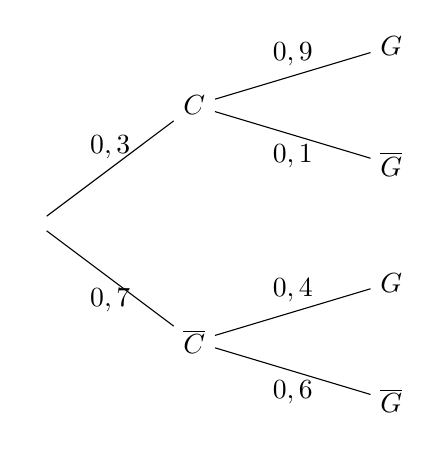
\begin{tikzpicture}
		[level 1/.style={level distance=2cm,
			sibling distance=3cm},
		level 2/.style={level distance=2.5cm,
			sibling distance=1.5cm}]
		\node {} [grow'=right]
		child {node {$C$}
			child {node {$G$}
				edge from parent node[above] {$0,9$}
			}
			child {node {$\overline G$}
				edge from parent node[below] {$0,1$}
			}
			edge from parent node[above] {$0,3$}
		}
		child {node {$\overline C$}
			child {node {$G$}
				edge from parent node[above] {$0,4$}
			}
			child {node {$\overline G$}
				edge from parent node[below] {$0,6$}
			}
			edge from parent node[below] {$0,7$}
		}
		;
	\end{tikzpicture}
\end{center}
	
	\subsection*{2.}
	

	\subsection*{3.}
	

	
	On a
	\[
	P(C \cap G) = P(C) \times P_C(G) = 0,3 \times 0,9 = 0,27.
	\]
	
	\subsection*{4.}
	

	D’après la loi des probabilités totales, on a :
	\[
	P(G) = P(C \cap G) + P(\overline{C} \cap G) = 0,3 \times 0,9 + 0,7 \times 0,4 = 0,27 + 0,28 = 0,55.
	\]
	
	\subsection*{5.}
	

	Il faut calculer \(P_G(C)\) :
	\[
	P_G(C) = \dfrac{P(G \cap C)}{P(G)} = \dfrac{P(C \cap G)}{P(G)} = \dfrac{0,27}{0,55} \approx 0,4909,
	\]
	
	soit 0,491 à \(10^{-3}\) près.
	
